\documentclass[11pt]{article}
\usepackage{hyperref}
\usepackage{graphicx}
\usepackage{caption}
\usepackage{geometry}
\usepackage{placeins}
\usepackage{enumitem}
\usepackage{multirow}
\usepackage{float}
\usepackage{wrapfig}
\usepackage{url}
\usepackage{amsmath}
\usepackage{algorithm}
\usepackage[backend=biber]{biblatex}
\usepackage{algpseudocode}
\usepackage{tikz}
\usepackage{schemata}
\usepackage{tabularx}
\usepackage{makecell}
\usepackage{pgfplots}
\usepackage[toc,page]{appendix}

\addbibresource{references.bib}



% Set page margins
\geometry{a4paper, margin=1.5cm}

% Set paragraph and spacing
\setlength{\parindent}{0em} % No indentation (annoying)
\setlength{\parskip}{0.5em} % Small space between paragraphs

\graphicspath{{../figures}}

\begin{document}

% TODO: update title
\begin{titlepage}
    \centering
    \vspace*{2cm}
    
    
    {\Huge\bfseries Fuzzy Expert System to Detect \\ Phishing in Websites\par}
    \vspace{1cm}
    % {\large A Comparative Analysis of k-Nearest Neighbors and SVM Classifiers\par}
    
    \vspace{2cm}
    
    {\large
    Dániel MÁCSAI \\ 
    Ismael RUIZ GARCIA \\ 
    Mauro VÁZQUEZ CHAS
    \par}
    
    \vspace{2cm}
    
    {\large
    \textbf{Master in Artificial Intelligence}
    \par}
    
    \includegraphics[width=0.4\textwidth]{Logo_URV.png}\par\vspace{1cm}

    \vspace{1cm}

    {\large
    Planning and Approximate Reasoning\\
    Delivery 3
    \par}
    
    \vspace{1cm}
    
    {\large\bfseries 15th December 2024\par}
    
\end{titlepage}


% Index
\newpage

\tableofcontents
\newpage

%---------------------------------------------------------------------------------------------------------------------------------
\section{Introduction}
For this work, we 
% TODO  write introduction

\section{Task 1}
To design the fuzzy expert system to detect phishing websites, we consulted ~\cite{mainpaper}. In this paper, they list 87 possible features (boolean, floats and integers) that could matter in the detection of phishing websites. The proposed features are divided into three categories: URL-based features, content features and external features. From this proposed variables, we selected 5 features that we consider relevant for the detection of phishing websites. For inspiration and further understanding of the problem, we consulted the following articles: \cite{introduction1} and \cite{introduction2}.

\subsection{Chosen Features}


\subsubsection{URL-based features:}
\textbf{Phish Hints} 
\begin{itemize}
    \item \textbf{Description} Number of words in the URL that are typical of phishing websites
    \item \textbf{Integer} Number 51 in the paper
\end{itemize}

\begin{figure}[H]
    \centering
    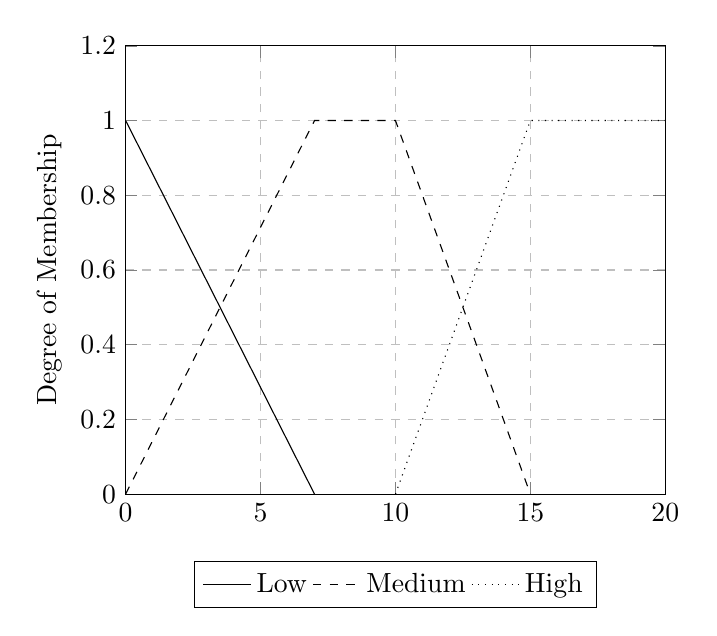
\begin{tikzpicture}
        \begin{axis}[
            ylabel={Degree of Membership},
            ymin=0, ymax=1.2,
            xmin=0, xmax=20,
            legend style={at={(0.5,-0.15)},anchor=north,legend columns=-1},
            ymajorgrids=true,
            xmajorgrids=true,
            grid style=dashed
        ]
        
        % Membership function for "Low"
        \addplot[solid, black] coordinates {(0,1) (0,1) (7,0)};
        \addlegendentry{Low}
        
        % Membership function for "Medium"
        \addplot[dashed, black] coordinates {(0,0) (7,1) (10,1) (15,0)};
        \addlegendentry{Medium}
        
        % Membership function for "High"
        \addplot[dotted, black] coordinates {(10,0) (15,1) (20,1)};
        \addlegendentry{High}
        
        \end{axis}
    \end{tikzpicture}
    \caption{Membership Function Phish Hints}
\end{figure}




\textbf{Domain Age} 
\begin{itemize}
    \item \textbf{Description:} Age of the page in months
    \item \textbf{Integer} Number 83 in the paper
\end{itemize}

\begin{figure}[H]
    \centering
    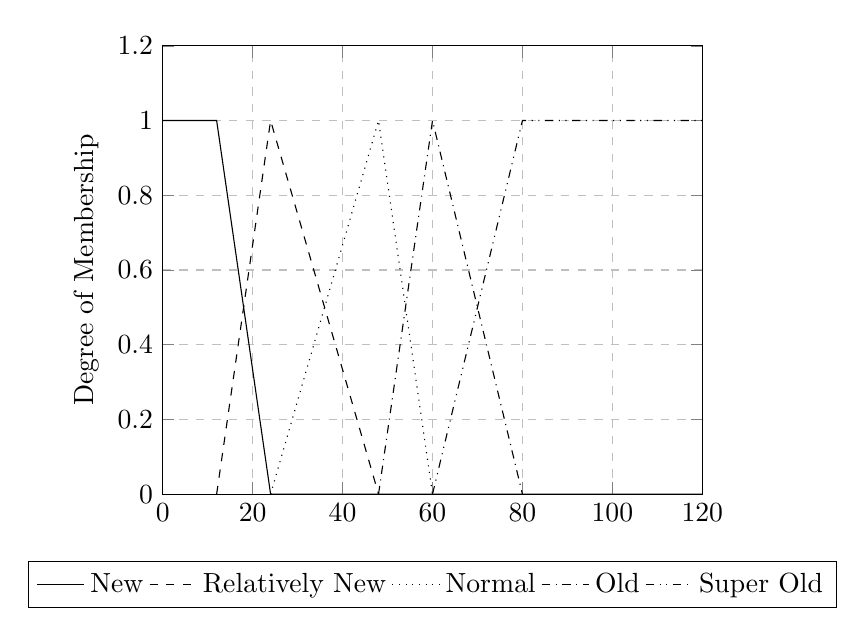
\begin{tikzpicture}
        \begin{axis}[
            ylabel={Degree of Membership},
            ymin=0, ymax=1.2,
            xmin=0, xmax=120,
            legend style={at={(0.5,-0.15)},anchor=north,legend columns=-1},
            ymajorgrids=true,
            xmajorgrids=true,
            grid style=dashed
        ]
        
        % Membership function for "New"
        \addplot[solid, black] coordinates {(0,1) (12,1) (24,0) (120,0)};
        \addlegendentry{New}
        
        % Membership function for "Relatively New"
        \addplot[dashed, black] coordinates {(12,0) (24,1) (48,0)};
        \addlegendentry{Relatively New}
        
        % Membership function for "Normal"
        \addplot[dotted, black] coordinates {(24,0) (48,1) (60,0)};
        \addlegendentry{Normal}
        
        % Membership function for "Old"
        \addplot[dash dot, black] coordinates {(48,0) (60,1) (80,0)};
        \addlegendentry{Old}
        
        % Membership function for "Super Old"
        \addplot[dash dot dot, black] coordinates {(60,0) (80,1) (120,1)};
        \addlegendentry{Super Old}
        
        \end{axis}
    \end{tikzpicture}
    \caption{Membership Function Domain Age (in months)}
\end{figure}



\subsubsection{Content features:}
\textbf{Ratio External Hyperlinks} 
\begin{itemize}
    \item \textbf{Description:} The number of external hyperlinks in a web page divided by the total number of hyperlinks
    \item \textbf{Float} Number 59 in the paper
\end{itemize}

\begin{figure}[H]
    \centering
    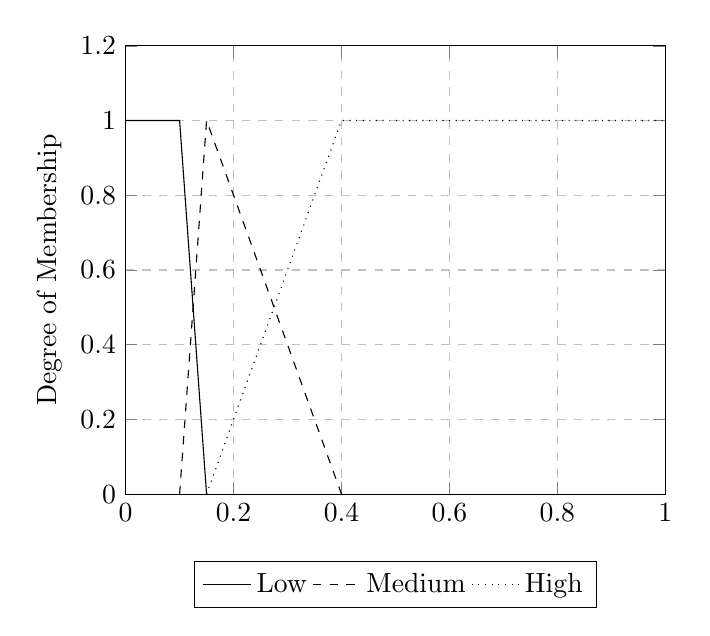
\begin{tikzpicture}
        \begin{axis}[
            ylabel={Degree of Membership},
            ymin=0, ymax=1.2,
            xmin=0, xmax=1,
            legend style={at={(0.5,-0.15)},anchor=north,legend columns=-1},
            ymajorgrids=true,
            xmajorgrids=true,
            grid style=dashed
        ]
        
        % Membership function for "Low"
        \addplot[solid, black] coordinates {(0,1) (0.1,1) (0.15,0)};
        \addlegendentry{Low}
        
        % Membership function for "Medium"
        \addplot[dashed, black] coordinates {(0.1,0) (0.15,1) (0.4,0)};
        \addlegendentry{Medium}
        
        % Membership function for "High"
        \addplot[dotted, black] coordinates {(0.15,0) (0.4,1) (1,1)};
        \addlegendentry{High}
        
        \end{axis}
    \end{tikzpicture}
    \caption{Membership Function Ratio External}
\end{figure}







\subsubsection{External features:}
\textbf{Google Index} 
\begin{itemize}
    \item \textbf{Description:} Whether a page is indexed in Google
    \item \textbf{Boolean} Number 86 in the paper
\end{itemize}

\begin{figure}[H]
    \centering
    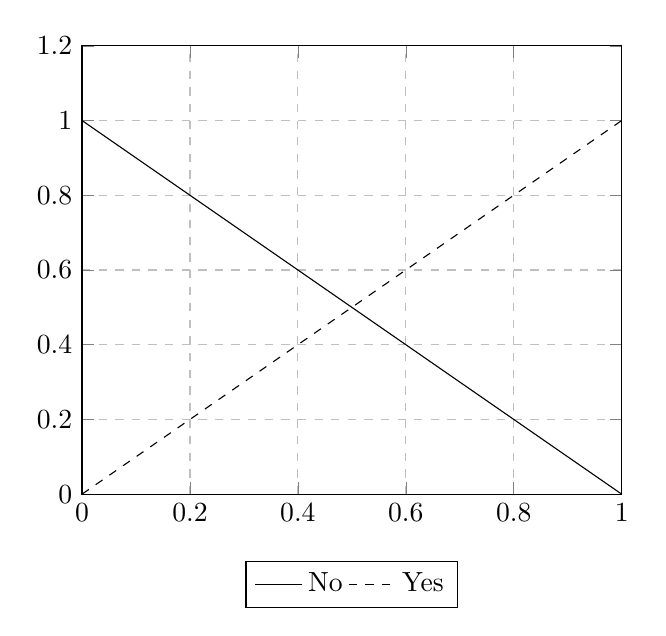
\begin{tikzpicture}
        \begin{axis}[
            ymin=0, ymax=1.2,
            xmin=0, xmax=1,
            legend style={at={(0.5,-0.15)},anchor=north,legend columns=-1},
            ymajorgrids=true,
            xmajorgrids=true,
            grid style=dashed
        ]
        
        % Membership function for "No"
        \addplot[solid, black] coordinates {(0,1) (1,0)};
        \addlegendentry{No}
        
        % Membership function for "Yes"
        \addplot[dashed, black] coordinates {(0,0) (1,1)};
        \addlegendentry{Yes}
        
        \end{axis}
    \end{tikzpicture}
    \caption{Membership Function Google Index}
\end{figure}





\textbf{GTR} 
\begin{itemize}
    \item \textbf{Description:} It is a slight modification of the usual GTR, created by Google. It means Google Toolbar Rank and takes values from 0 to 10.
    \item \textbf{Integer} Number 87 in the paper
\end{itemize}

\begin{figure}[H]
    \centering
    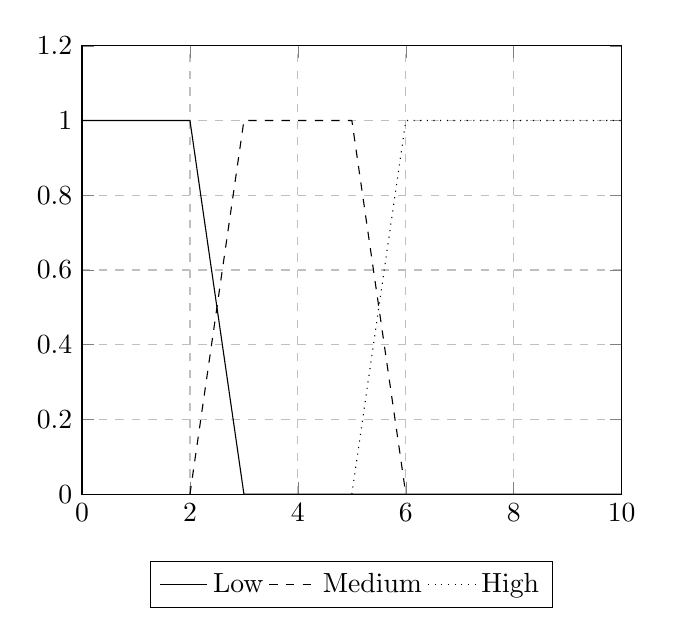
\begin{tikzpicture}
        \begin{axis}[
            ymin=0, ymax=1.2,
            xmin=0, xmax=10,
            legend style={at={(0.5,-0.15)},anchor=north,legend columns=-1},
            ymajorgrids=true,
            xmajorgrids=true,
            grid style=dashed
        ]
        
        % Membership function for "Low"
        \addplot[solid, black] coordinates {(0,1) (2,1) (3,0) (10,0)};
        \addlegendentry{Low}
        
        % Membership function for "Medium"
        \addplot[dashed, black] coordinates {(2,0) (3,1) (5,1) (6,0)};
        \addlegendentry{Medium}
        
        % Membership function for "High"
        \addplot[dotted, black] coordinates {(5,0) (6,1) (10,1)};
        \addlegendentry{High}
        
        \end{axis}
    \end{tikzpicture}
    \caption{Membership Function Google GTR}
\end{figure}



\section{Output Variable}
Our output variable will be the phishing risk, where we will consider 5 different fuzzy sets, see \ref{output_variable}.

\begin{figure}[H]
    \centering
    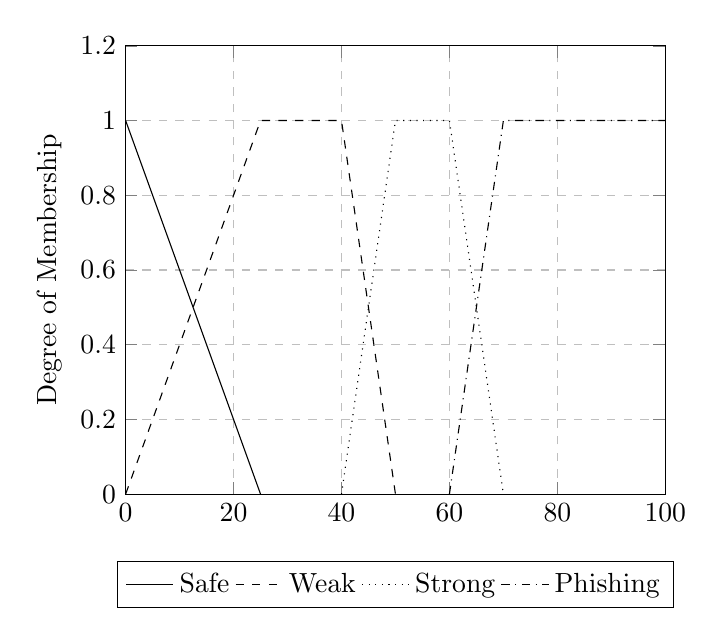
\begin{tikzpicture}
        \begin{axis}[
            ylabel={Degree of Membership},
            ymin=0, ymax=1.2,
            xmin=0, xmax=100,
            legend style={at={(0.5,-0.15)},anchor=north,legend columns=-1},
            ymajorgrids=true,
            xmajorgrids=true,
            grid style=dashed
        ]
        
        % Membership function for "Safe"
        \addplot[solid, black] coordinates {(0,1) (0,1) (25,0)};
        \addlegendentry{Safe}
        
        % Membership function for "Weak"
        \addplot[dashed, black] coordinates {(0,0) (25,1) (40,1) (50,0)};
        \addlegendentry{Weak}
        
        % Membership function for "Strong"
        \addplot[dotted, black] coordinates {(40,0) (50,1) (60,1) (70,0)};
        \addlegendentry{Strong}
        
        % Membership function for "Phishing"
        \addplot[dash dot, black] coordinates {(60,0) (70,1) (100,1)};
        \addlegendentry{Phishing}
        
        \end{axis}
    \end{tikzpicture}
    \caption{Membership Function Phishing Risk (Output Variable)}
    \label{output_variable}
\end{figure}




% ----------------
\section{Rules}

To design the rules involving Google Index, we consulted ~\cite{mainpaper}, where they state that pages not indexed by google are more likely to be phishing websites. For this reason we created the rules in \ref{google_index_rules}.

\begin{table}[H]
    \centering
    \begin{tabular}{|l|l|l|}
        \hline
        \textbf{Google Index} & \textbf{Phishing Risk} & \textbf{Weight} \\ \hline
        NO                    & PHISHY                 & 1               \\ \hline
        YES                   & WEAK                   & 1               \\ \hline
    \end{tabular}
    \caption{Rules for Google Index}
    \label{google_index_rules}
\end{table}

For the GTR, we consulted ~\cite{GTR}, where they state the following:

\begin{quote}
    \textit{GTR value is considered as a heuristic because PageRank value for legitimate site will be high and for phishing pages its value will be less}
\end{quote}

In the case of the Phish Hints, it is already explained in ~\cite{mainpaper} that more Phish Hints in the URL is an indicator of a phishing website. For this reason, we introduced the rules in Table \ref{page_rank_phish_hints_rules}.

\begin{table}[h]
    \centering
    \begin{tabular}{|l|l|l|l|l|}
    \hline
    \textbf{GTR} & \textbf{Phis Hints} & \textbf{Operator} & \textbf{Phishing Risk} & \textbf{Weight} \\ \hline
    HIGH               &                     &                   & SAFE                   & 1               \\ \hline
    MEDIUM             & LOW                 & AND               & WEAK                   & 0.5             \\ \hline
    MEDIUM             & MEDIUM              & AND               & STRONG                 & 1               \\ \hline
    MEDIUM             & HIGH                & AND               & PHISHY                 & 1               \\ \hline
    LOW                & LOW                 & AND               & STRONG                 & 0.5             \\ \hline
    LOW                & MEDIUM              & AND               & STRONG                 & 1               \\ \hline
    LOW                & HIGH                & AND               & PHISHY                 & 1               \\ \hline
    \end{tabular}
    \caption{Rules for Google GTR and Phish Hints}
    \label{page_rank_phish_hints_rules}
\end{table}


To evaluate the effect of the domain age feature, we consulted ~\cite{domainage}, where they state the following:

\begin{quote}
\textit{The top feature in the list is domain age, which confirms our assumptions that long-running services are statistically more credible}
\end{quote}

For this reason, we will consider that the older the domain, the less likely it is to be a phishing website. On the other hand, to evaluate the effect of the ratio of external hyperlinks, we consulted ~\cite{externalhyperlinks}, where the following is affirmed:

\begin{quote}
\textit{Phishing websites often include numerous external hyperlinks pointing to target websites because cybercriminals frequently replicate the HTML code from legitimate websites to construct their phishing sites.}
\end{quote}

All of this information, lead to the creation of the rules seen in Table \ref{domainage_hyperlinks_rules}.

\begin{table}[H]
    \centering
    \begin{tabular}{llllll}
                          &                                     &                                          &                               &                                    &                             \\ \cline{2-6} 
    \multicolumn{1}{l|}{} & \multicolumn{1}{l|}{\textbf{Domain Age}}     & \multicolumn{1}{l|}{\textbf{Ratio of Hyperlinks}} & \multicolumn{1}{l|}{\textbf{Operator}} & \multicolumn{1}{l|}{\textbf{Phishing Risk}} & \multicolumn{1}{l|}{\textbf{Weight}} \\ \cline{2-6} 
    \multicolumn{1}{l|}{} & \multicolumn{1}{l|}{SUPER OLD}      & \multicolumn{1}{l|}{}                    & \multicolumn{1}{l|}{}         & \multicolumn{1}{l|}{SAFE}          & \multicolumn{1}{l|}{1}      \\ \cline{2-6} 
    \multicolumn{1}{l|}{} & \multicolumn{1}{l|}{OLD}            & \multicolumn{1}{l|}{LOW}                 & \multicolumn{1}{l|}{OR}       & \multicolumn{1}{l|}{SAFE}          & \multicolumn{1}{l|}{0.5}    \\ \cline{2-6} 
    \multicolumn{1}{l|}{} & \multicolumn{1}{l|}{NORMAL}         & \multicolumn{1}{l|}{LOW}                 & \multicolumn{1}{l|}{AND}      & \multicolumn{1}{l|}{WEAK}          & \multicolumn{1}{l|}{0.5}    \\ \cline{2-6} 
    \multicolumn{1}{l|}{} & \multicolumn{1}{l|}{NORMAL}         & \multicolumn{1}{l|}{MEDIUM}              & \multicolumn{1}{l|}{AND}      & \multicolumn{1}{l|}{STRONG}        & \multicolumn{1}{l|}{0.5}    \\ \cline{2-6} 
    \multicolumn{1}{l|}{} & \multicolumn{1}{l|}{NORMAL}         & \multicolumn{1}{l|}{HIGH}                & \multicolumn{1}{l|}{AND}      & \multicolumn{1}{l|}{STRONG}        & \multicolumn{1}{l|}{0.5}    \\ \cline{2-6} 
    \multicolumn{1}{l|}{} & \multicolumn{1}{l|}{RELATIVELY NEW} & \multicolumn{1}{l|}{LOW}                 & \multicolumn{1}{l|}{AND}      & \multicolumn{1}{l|}{WEAK}          & \multicolumn{1}{l|}{1}      \\ \cline{2-6} 
    \multicolumn{1}{l|}{} & \multicolumn{1}{l|}{RELATIVELY NEW} & \multicolumn{1}{l|}{MEDIUM}              & \multicolumn{1}{l|}{AND}      & \multicolumn{1}{l|}{STRONG}        & \multicolumn{1}{l|}{1}      \\ \cline{2-6} 
    \multicolumn{1}{l|}{} & \multicolumn{1}{l|}{RELATIVELY NEW} & \multicolumn{1}{l|}{HIGH}                & \multicolumn{1}{l|}{AND}      & \multicolumn{1}{l|}{PHISHY}        & \multicolumn{1}{l|}{0.5}    \\ \cline{2-6} 
    \multicolumn{1}{l|}{} & \multicolumn{1}{l|}{NEW}            & \multicolumn{1}{l|}{LOW}                 & \multicolumn{1}{l|}{AND}      & \multicolumn{1}{l|}{STRONG}        & \multicolumn{1}{l|}{0.5}    \\ \cline{2-6} 
    \multicolumn{1}{l|}{} & \multicolumn{1}{l|}{NEW}            & \multicolumn{1}{l|}{MEDIUM}              & \multicolumn{1}{l|}{AND}      & \multicolumn{1}{l|}{STRONG}        & \multicolumn{1}{l|}{1}      \\ \cline{2-6} 
    \multicolumn{1}{l|}{} & \multicolumn{1}{l|}{NEW}            & \multicolumn{1}{l|}{HIGH}                & \multicolumn{1}{l|}{AND}      & \multicolumn{1}{l|}{PHISHY}        & \multicolumn{1}{l|}{1}      \\ \cline{2-6} 
    \end{tabular}
    \caption{Rules for Domain Age and Ratio of External Hyperlinks}
    \label{domainage_hyperlinks_rules}
\end{table}




\section{Implementation}
In our implementation, we utilized the MATLAB Fuzzy Logic Toolbox to develop the fuzzy expert system. The system was designed using the Mamdani fuzzy inference method, which is well-suited for decision-making processes that require a human-like reasoning approach. In this system, we employed the minimum (min) operation as the t-norm for the intersection of fuzzy sets, and the maximum (max) operation as the t-conorm for the union of fuzzy sets. For the defuzzification process, we selected the Center of Area (CoA) method, which calculates the centroid of the aggregated fuzzy set to produce a crisp output. This approach ensures that the output is a balanced representation of the input conditions, providing a reliable decision-making framework for detecting phishing websites.

To validate the fuzzy expert system, we employed the MATLAB 3D plot. As this plot only allows the representation of 2 inputs and the output at a time, we viewed the 10 possible combinations, all of which were consistent. At the same time, every possible combination was covered, as no combination was left without a rule being activated.

\section{Testing}
- 4 Test case that represent different situation (some must activate more than one lable)
- Report the results of each testing case with 
screenshots  and  explanations  that  justify the output  obtained  (i.e.  showing  the  activations of  
rules)

We test it for the following cases:
Phising: 
https://dichvuvnpt.com/home/components/com_user/bbtonline.html

Phish hints: 0
Domain Age: 3767
Ratio External Hyperlinks: 1.0
Google Index: 1
Page rank: 0

\section{Complex Fuzzy Expert System}
Design (just graphically, no implementation) a more complete fuzzy expert system that 
includes more features about the websites. Show in a figure the inputs, outputs, and rule blocks 
that you propose for such expert system. No specific definition of variables nor rules is required. 

- We can use a hierarchical rule system

% Bibliography
\newpage
\printbibliography


\end{document}